\documentclass[11pt]{article}
\usepackage[left=3cm,right=3cm,top=3cm,bottom=3cm]{geometry}
\usepackage[utf8]{inputenc}
\usepackage[T1]{fontenc}
\usepackage{amsmath}
\usepackage{amssymb}
\usepackage{hyperref}
\usepackage{graphicx}
\usepackage{xcolor,listings}
\usepackage{siunitx}
\usepackage[ruled,linesnumbered]{algorithm2e}
\sisetup{range-phrase=--}
\sisetup{range-units=single}

\usepackage{titling}
\setlength{\droptitle}{-6em}


% Used to reference java classes
\newcommand{\class}[1]{{\color{green!50!black}\small\texttt{#1}}}
% Used to reference files or folders in the git/project directory
\newcommand{\source}[1]{{\color{blue!80!white}\texttt{\lstinline|#1|}}}



\title{Project Report: BamBirds 2018\\
{\small Creating an Intelligent Game Playing Agent for Angry Birds}}

\author{
David\\Hollinger
\and Diedrich\\Wolter
\and Felix\\Schweinfest
\and Harshit\\Kumar Gupta
\and Jan\\Martin
\and Johanna\\Seibert
\and Lara\\Aubele
\and Oleg\\Geier
}


\def\maketitlehookb{
\begin{center}

\includegraphics[width=50mm]{img/logo.png}
\end{center}
}

\begin{document}
\maketitle
\tableofcontents
\section{Aufgabenstellung des Smart Environment Projekts}
AngryBirds, ein in 2009 von Rovio Entertainment entwickeltes Casual-Puzzle-Videospiel, ist ideal als Maßstab für künstliche Intelligenz geeignet. Der Weg zum Erfolg setzt voraus, dass ein Verständnis der physikalischen Zusammenhänge auf das Spiel übertragen werden können und strategische Entscheidungen getroffen werden müssen. Ziel des Projekts war es, die Schwächen des BamBirds-Agenten zu verbessern und um Funktionen zu erweitern, um mit diesem an der Angry Birds AI Competition teilnehmen zu können und diesen zu gewinnen.\\Parallel zu diesem Wettkampf, lief die sogenannte AIBirds COG 2019 Level Generation Competition, in welchem das Ziel daraus bestand, mit einem selbsterstellten Programm der Wahl, automatisiert Level zu generieren, welche viel Spaß und Herausforderung anbieten sollen. Dieser Aufgabe haben wir uns gewidmet.
\section{Level Editor}\label{ch:leveleditor}
\subsection{Manual Levelgenerator}
\subsubsection{Preexisting Levelgenerator}
As a base we used an already existing leveleditor\footnote{http://www.battlefieldsingleplayer.com/apachethunder/angrybirds/} which works by selecting from a number of objects and positioning them with the keyboard.
By pressing save the level is downloaded as Lua file. 
\subsubsection{Parser for Format Change}
We wrote a parser that takes all levels from the levelsToParse folder and converts them to json files.
If 'Bird' was in the original level format (Lua file) we concatenated 'bird\_' and the number of the bird otherwise we the key was 'block\_' and the number of the block.
The position in the original format and the position in the game we needed was not the same so we multiplied it with 0.91 which differs if you start to zoom into the levelgenerator and position the blocks closer to each other. Then the 0.91 can be removed. The parser also adds 52 to the x value of the blocks and put all birds behind the slingshot.
The blocks in the levelgenerator can be turned in either way and result in different angles depending if they were turned to the right (positive radian) or to the left (negative radian). We converted them to positive degree values.
The names of the blocks, pigs and the birds differ as well in the two formats, we solved this with a dictionary where the names from the lua file are the key and the names of our version are the values. The parser then chooses the value for the found key from the Lua file to get the name of the structure, bird or pig. We convert the longest breakable structure block to terrain as this structure block does not exist in the version of the game that we use.
The parser also removes the preexisting blocks and the pig of the editor. We added code to remove the birds aswell but they are currently commented out so this can be adapted if the user wishs to remove the birds, too.
After converting the content which is described above the prefile.json which contains the additional necessary json code is added as well as the number of blocks and birds.
The place where the converted level is saved is parsedLevels per default. This can be changed to the slingshot folder of the game in the parser. 

\subsubsection{How to Use the Manual Levelgenerator}
\begin{enumerate}
	\item \textbf{Open the Editor Locally}
	
	Go to the directory `levelGenerator/manualLevelGeneratorJS/` and open the index.html in your webbrowser.
	\item \textbf{Create the Level}
	
	Create the level you want, you can put the birds where you want as they will moved to the correct position anyways. You can use \textbf{all kinds of birds and pigs} in the game. The other things you can use are limited to \textbf{all blocks of stone, ice, wood, static breakable structure and terrain}. The latest two look same in the editor but can be differentiated through the code on the top of the page.
	You can position the blocks and pigs from the very left side of the window to the very right side. It is better to not zoom in, which is possible with the up and down arrow key, as the factor of 0.91 would not fit anymore and the very left side could not be used to place objects anymore. The factor with zooming in could be 1 for example. This is the case because then the objects fit closer together so if you put two items right next to each other they would be closer together than without zooming in. When the factor is not adapted in this case, the objects are too close together and structures can collapse.
	Most of the hints for editing are already given in the editor itself. To delete objects you only have to press the delete key.
	
	\item \textbf{Save Level} Click at save and save the level to a folder.
	
	\item \textbf{Adapt Paths} Open the Parser.py and adapt all paths to your personal structure (optional: only if not already done before).

	\item \textbf{Run Parser} Run the Parser.py with python3

	\item \textbf{Copy File} If you did not change the structure of the output-file to the json directory where you run your game \footnote{if you run the game in slingshot this would be in `cors/fowl/json/`} copy the file now in this directory (optional: only if not changed before)

	\item \textbf{Run Game} Run Angrybirds (now you should see the new level you just created, if this is not the case check if your machine cached the levels)
	
\end{enumerate}

\subsection{Random Levelgenerator}
\label{Random LevelGenerator}
\subsubsection{General}
	The random levelgenerator can create different kinds of levels. The number of the levels of the different types can be changed in the main class:
	\begin{description}
		\item[Main](\class{levelGenerator.main})\\
			The main method calls the createLevel methods with the number of levels that should be generated. 
		\item[LevelCreator](\class{levelGenerator.LevelCreator})\\
			This class calls the create method of the BasicLevel with the parameter and the type of level that was requested. In addition to the level types below it can generate a simple level where the Basic Level is called with no structure to add.
		\item[BasicLevel](\class{levelGenerator.LevelCreator})\\
			Adds the basic things the LevelN-M.json file needs to actually work as level like f.e. the camera.
			It also adds as many randomized blocks, pigs, terrainblocks as the method was called with as well as the structure and the red birds.
			This class can also receive a list with all positions of the blocks of the structure and put the blocks around it. This feature does not work for all kinds of levels yet. 
	\end{description}
\subsubsection{Structure Levels}
\begin{description}
	\item[DominoLevel](\class{levelGenerator.DominoStructure})\\
		The level contains three vertical large blocks that are positioned on the ground and their distance and material is picked randomly. The distance and the material is for all blocks the same. For this level the pigs and a chosen amount of random blocks are positioned randomly by the LevelCreator class.
		\begin{figure}[tbh!]
			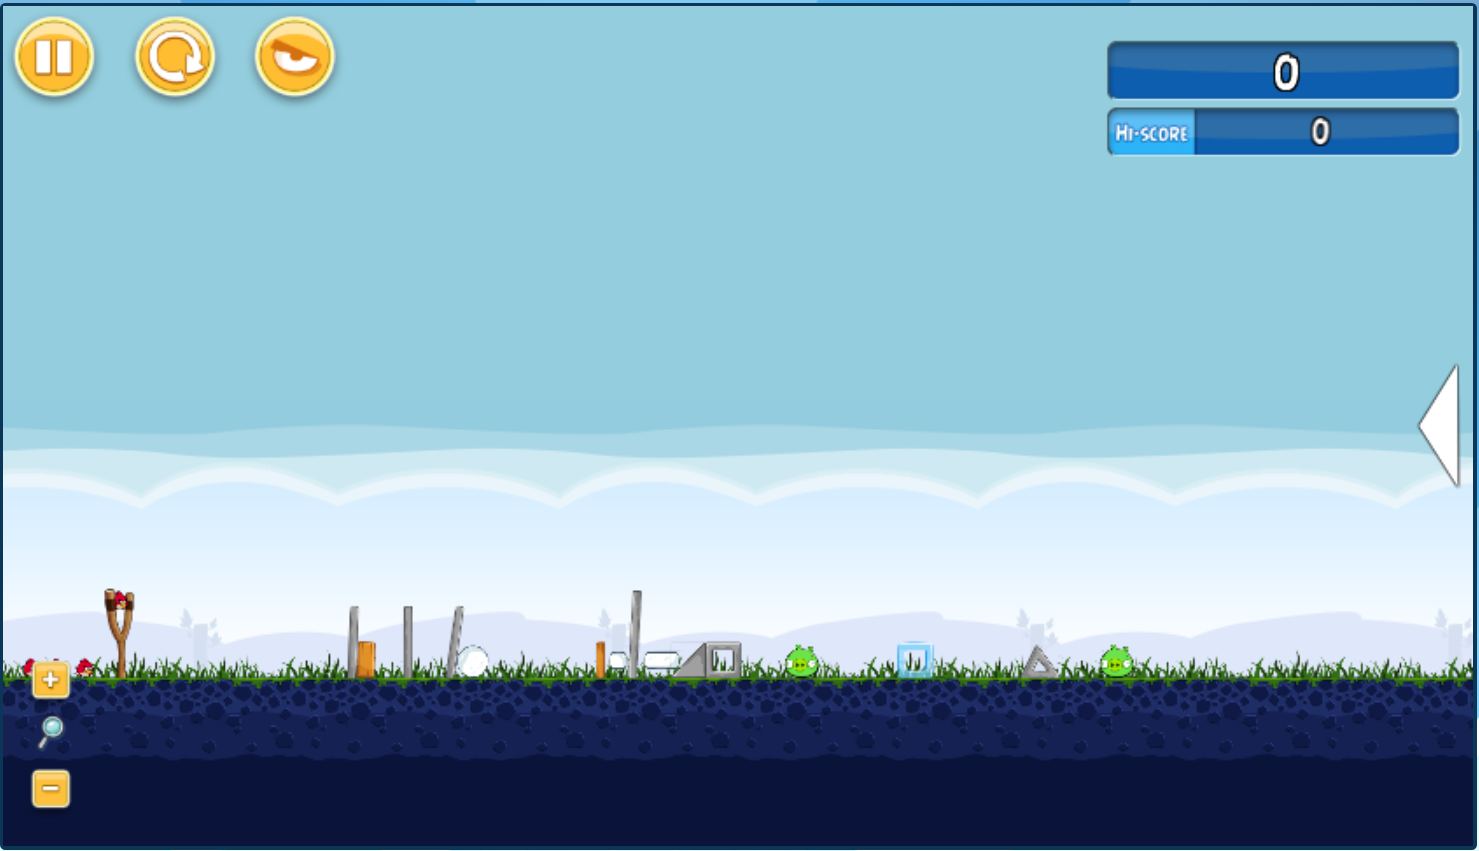
\includegraphics[width=0.5\textwidth]{img/DominoLevel.png}
			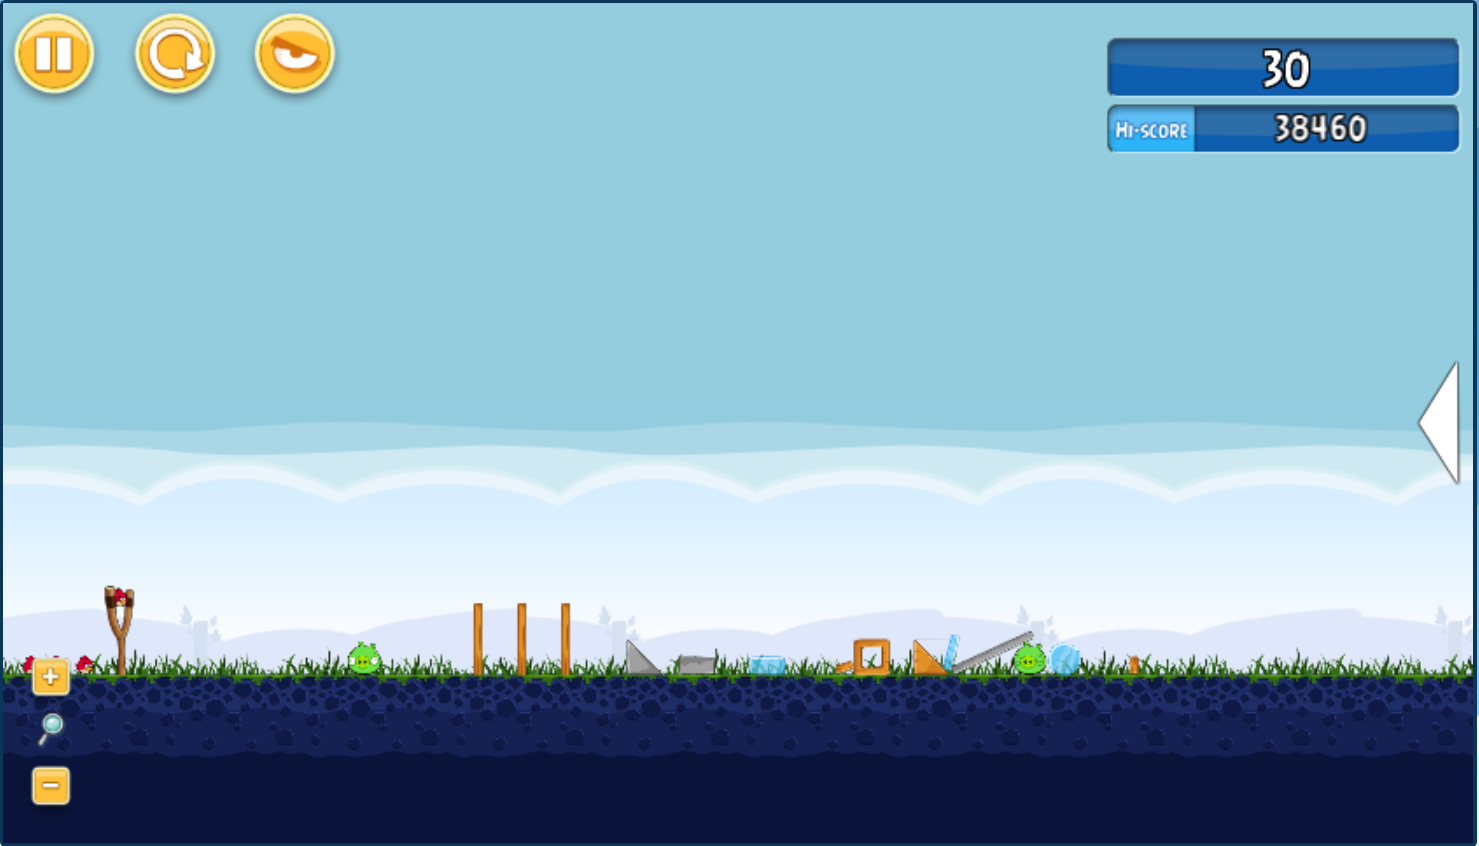
\includegraphics[width=0.5\textwidth]{img/DominoLevel2.png}
			\caption{Two examples of DominoLevels}
		\end{figure}
	\item[HouseLevel](\class{levelGenerator.HouseStructure})\\
		In this level houses build out of three long blocks are created. The structure can randomly be either on the ground or on a static block in the air. Where the structure is and what material it is build of depends on the random values. The material of all blocks is the same and only large blocks can be chosen. The first level of the structure can have up to three houses and can have a second level with one house less. The pigs positioned in the level are all the same but picked randomly and positioned in each house of the first level of the structure.
		\begin{figure}[tbh!]
		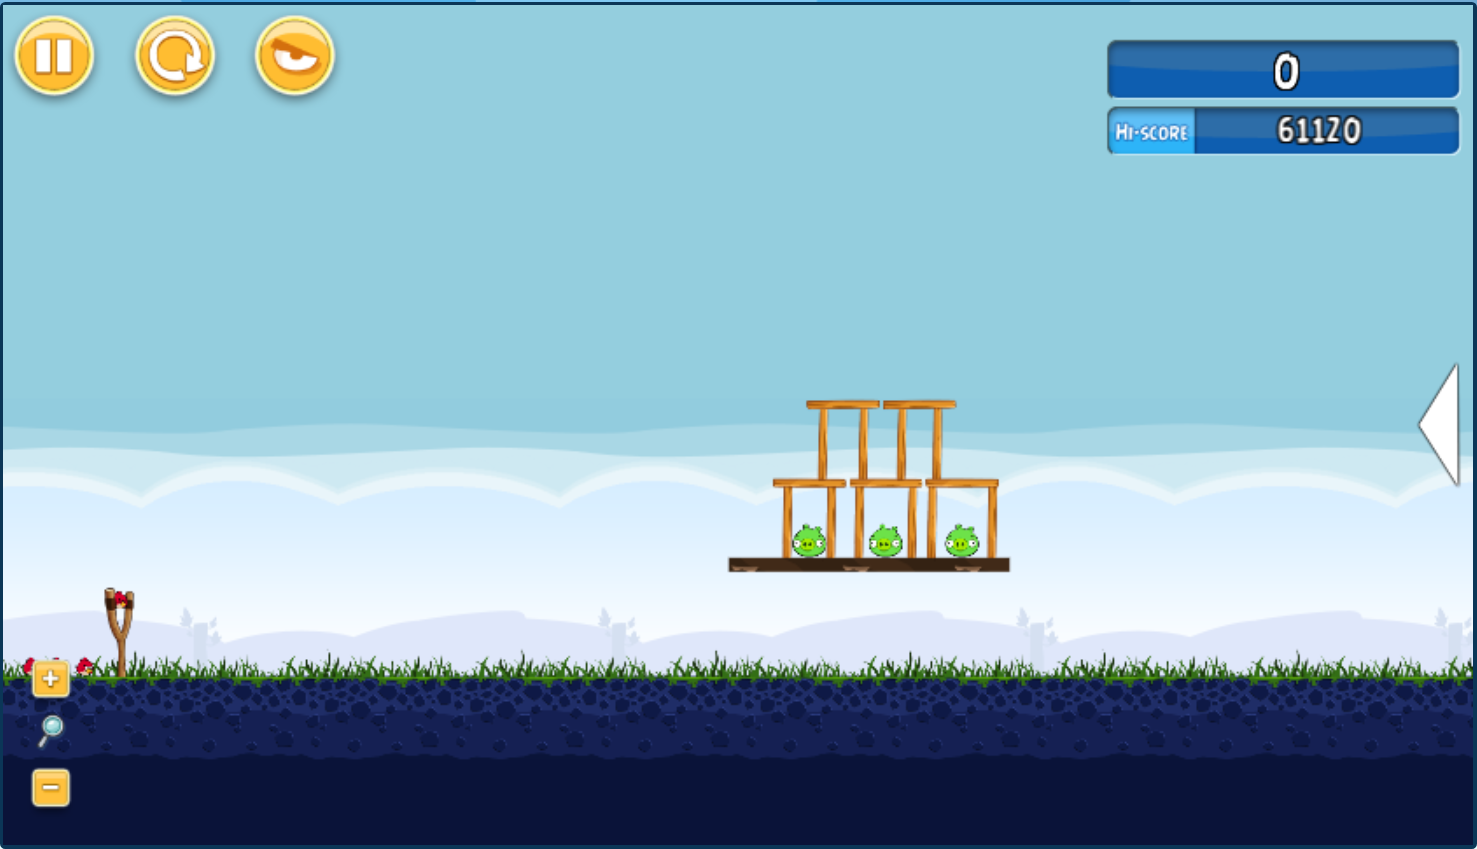
\includegraphics[width=0.5\textwidth]{img/HouseLevel.png}
		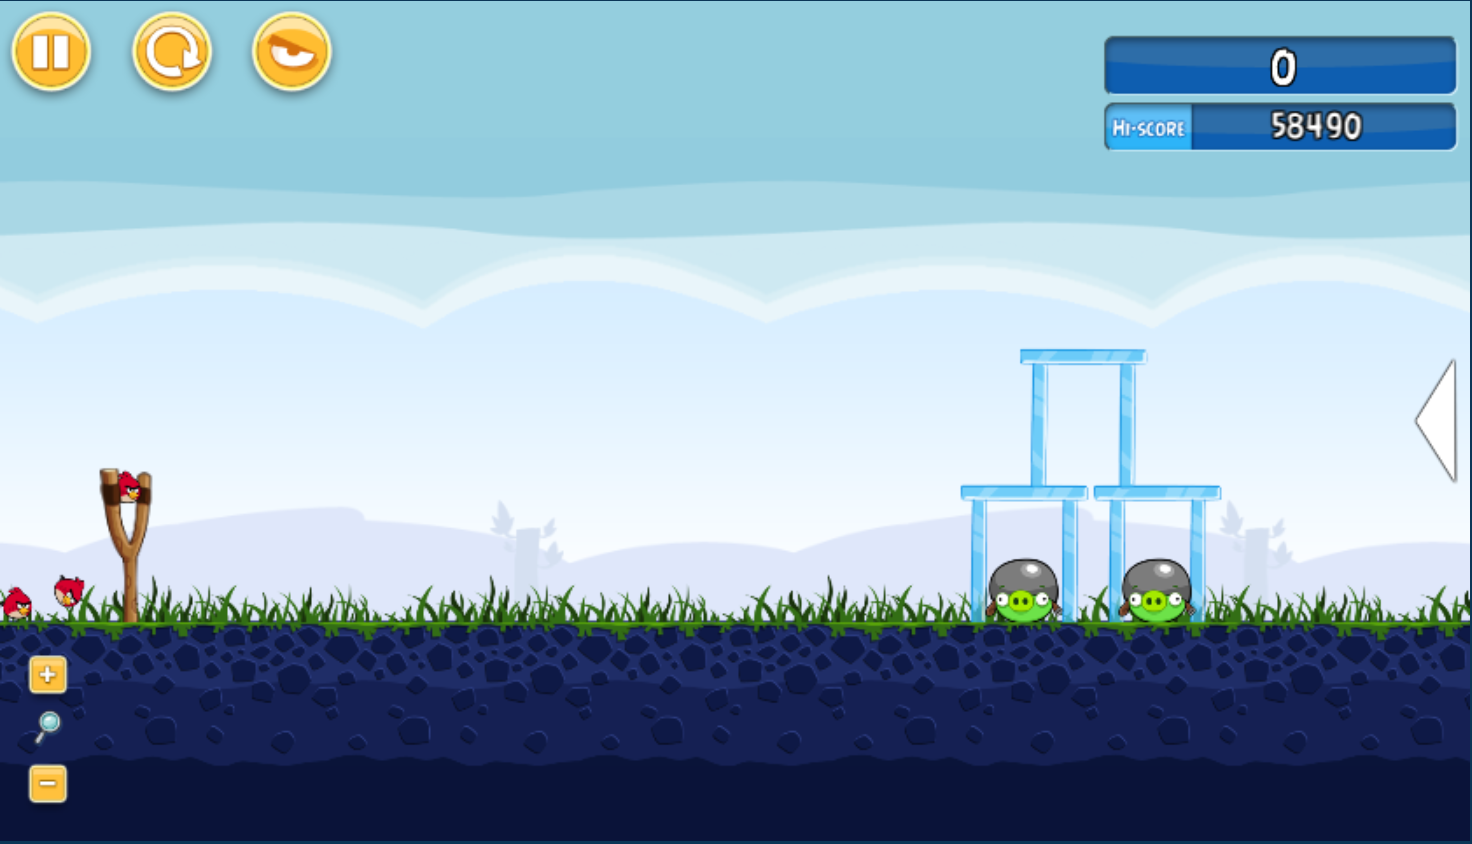
\includegraphics[width=0.5\textwidth]{img/HouseLevel2.png}
		\caption{Two examples of HouseLevels}
		\end{figure}
	\item[FunnelLevel](\class{levelGenerator.FunnelStructure})\\
		For this kind of level a static block is positioned horizontally above the ground so a bird still fits below. At the end of this funnel there is a pig. Random blocks can be positioned all over the level by the LevelCreator class.
		\begin{figure}[tbh!]
			\centering
			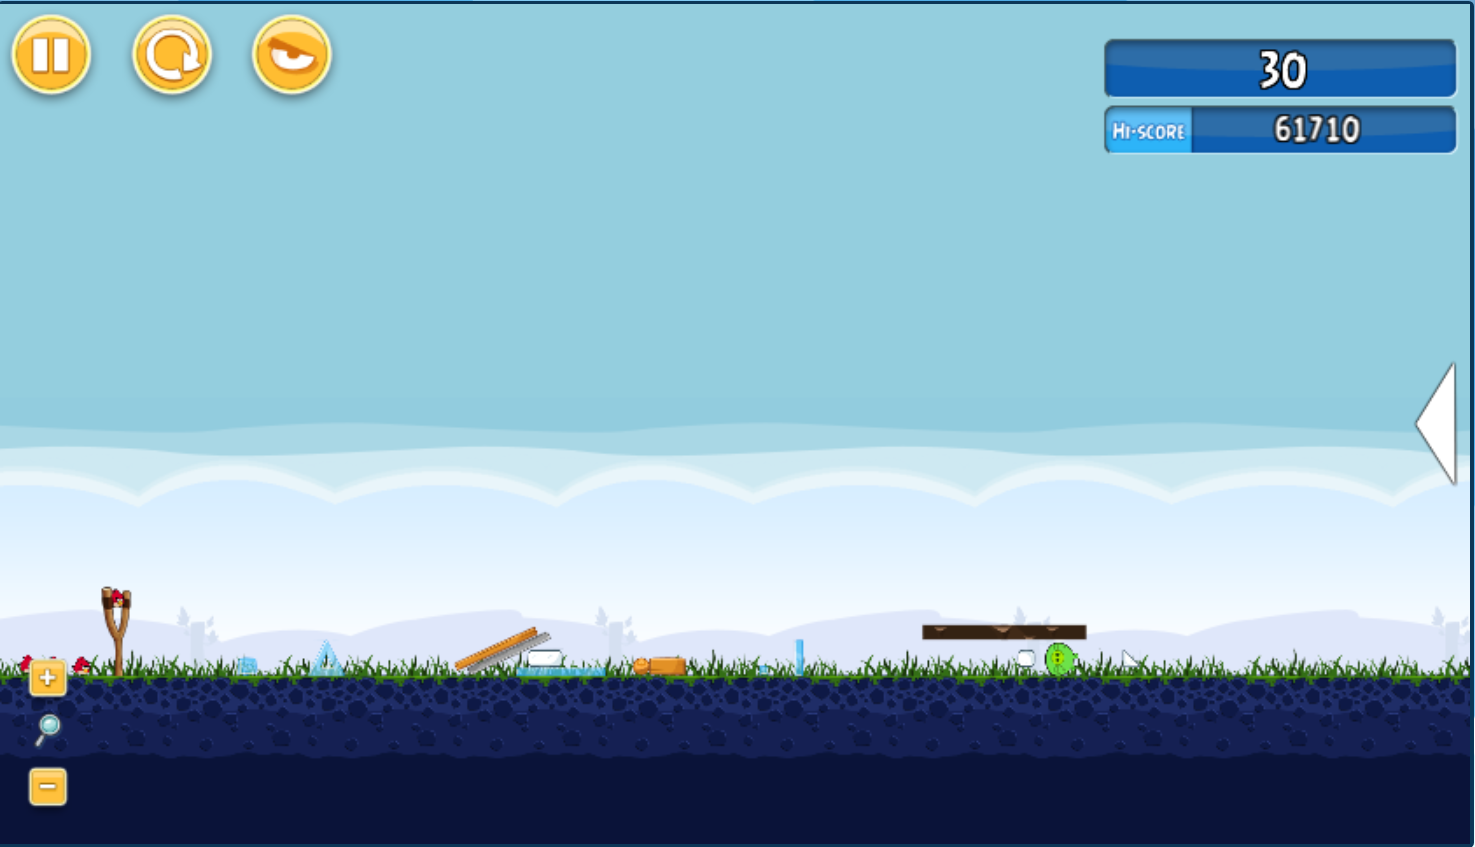
\includegraphics[width=0.5\textwidth]{img/FunnelLevel.png}
			\caption{An example of a FunnelLevel}
		\end{figure}
		\end{description}
\subsubsection{How to Use the Random Levelgenerator}
	\begin{enumerate}
		\item \textbf{Select Levels} Open the Main class and comment/uncomment the calling of the create*-functions in the main method according to the type of levels you want to create. Change the parameter of those method calls to the number of levels you want to create of this type.
		\item \textbf{Run Generator} Run main.java
		\item \textbf{Copy File} Copy the levels to the directory where you want to play the game (json directory), make sure you use only levels of one type at the time or rename them properly (Level1-\textit{1 to 21}.json)\footnote{for example Level1-4.json}. The first number is the page and the second is the level of the page.
		\item \textbf{Run Game} Run Angrybirds
	\end{enumerate}
\subsection{Transformation Values for Editing .json Level Files}

Assuming the x-value for a block in the LevelN-M.json is called \textit{json.x}, and the x-value of the MBR-vision-module is called \textit{mbr.x}, the formula for transforming json.x to mbr.x is: 
\[mbr.x = json.x * 5 + 14\]

Remember that mbr.x (and mbr.y) marks the x-value (and y-value) of the \textit{upper left corner} of the block. The RealShape vision module however returns the \textit{center-values} of each block. 

With the y-values, it is a bit more difficult, since there might be blocks underneath the block that \textit{lower} mbr.y. The baseline (ground line of the level) in the vision-module is 385. Each block-y-value (let that be json.y, e.g. 4 on a vertically aligned WOOD\_BLOCK\_4X1) \textbf{lowers the baseline by 5}, so, the higher the block is, the lower the number gets. A vertically aligned WOOD\_BLOCK\_10X1 has a mbr.y of 335 (`385 - 5 * json.y = mbr.y`), while a vertically aligned WOOD\_BLOCK\_4X1 has a mbr.y of 365.
\section{Evaluation}\label{ch:evaluation}

\subsection{Evaluation Framework}
In order to make the evaluation of our agent easier and less time-consuming, we build an evaluation framework capable of automated running agents and analysis of the performance. Doing that, it is possible to compare the performance of our agent at the current state of development with the other teams' agents made publicly available on the aibirds forum. Having the possibility to easily evaluate the agent helps to detect problems with specific levels, but more important, it shows whether changes made to the code affect the performance of the agent on levels where it was not expected. \\
The evaluation framework consists of three parts, each of it wrapped into an own class: The class main defines the command line user interface, which can be used to choose the levels and agents. The class automatically copies the desired levels into the level folder of the game, such that those levels are loaded when the game is started. There are all levels of the previous competitions available. Also, it is possible to load levels generated by yourself (this can be done by using the level generator). \\
The class logger is responsible for starting the game, starting the agents on the desired levels and logging the achieved scores. The logging is implemented by filtering the console output of ABServer. The results are stored into an csv-file. The class logs continuously, so it is possible to have a look at the performance while the test is still running.\\
Finally, the class evaluator offers an command line user interface and the logic for analyzing the logged scores of the agents and generating bar charts which show the performance of the agents. As a result, a pdf file is created which holds 3 kinds of bar charts for every level: First, a chart which shows the mean score of an agent, e.g., the average score of an agent over all runs of the level. The second chart shows the median of the scores. The last type shows the highest score (max-score) an agent has achieved on the specific level. This one is the most important chart, because if the evaluation is conducted under competition conditions, the highest score is the only one that counts. Additionally, there is a chart at the end of the pdf which shows the sums of all highest scores. This is also the measurement used in the finals of the competition.\\
The evaluation framework was entirely written in python. This allowed us to write compact, easy-to-read code. Python also allows an uncomplicated access to data analysis tools and, as a scripting language, is more suitable for pipeline-like architectures than Java. \\
Examples of the charts generated by evaluator.py can be found in figure \ref{fig:output1} and \ref{fig:output2}

\begin{figure}%[t] 
	\centering 
	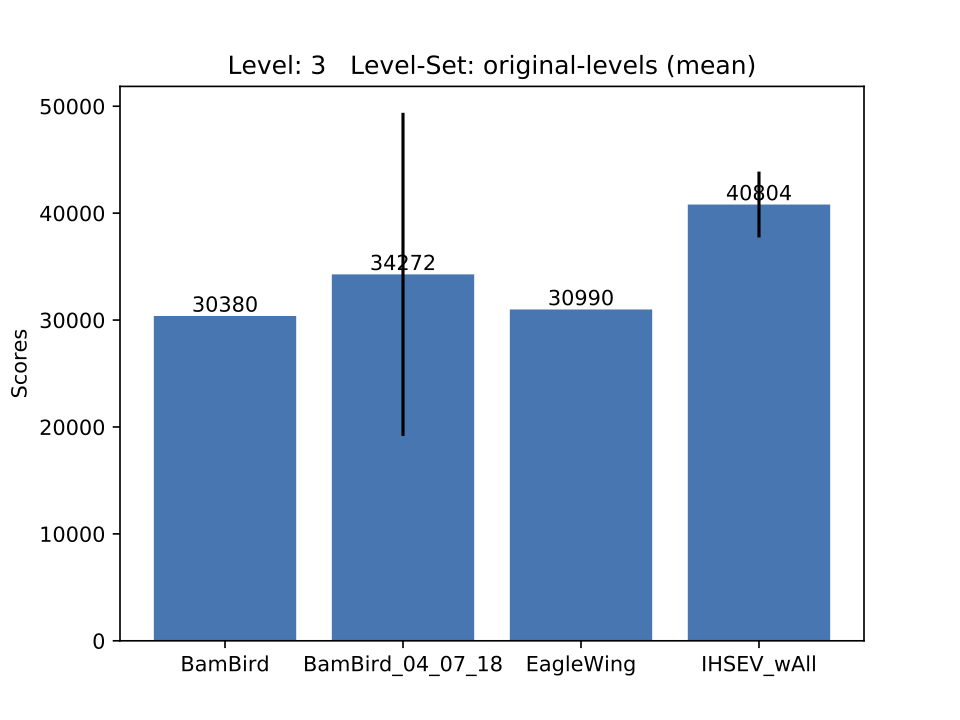
\includegraphics[width=50mm]{img/evaluation_results_05_07_18_11_20_33_original_levels.png}
	\caption{The evaluation of a preliminary BamBird 2018 agent against other teams' agents on the third level of the original levels (Poached Eggs). The bar chart shows the agents' average score on the level.\label{fig:output1}}
\end{figure}

\begin{figure}%[t] 
	\centering 
	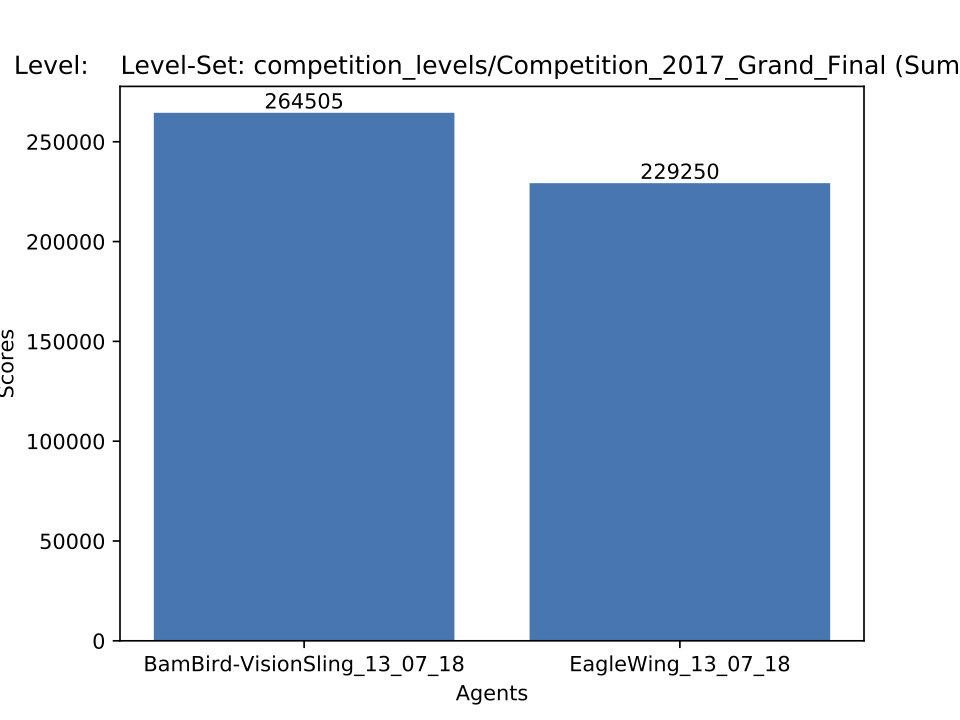
\includegraphics[width=50mm]{img/evaluation_results_13_07_18_21_17_06_grand_final_2017.png}
	\caption{The evaluation of the final BamBird agent against EagleWing 2017 on the grand final of 2017. The chart shows the sum of the highest score of every on all 8 levels.\label{fig:output2}}
\end{figure}

\subsection{Evaluation results}
In order to evaluate the final agent, we performed a benchmark which consisted of a 60 minutes run on the first stage of the Poached Eggs levels. While the agent of 2017 scored 663940 points in this benchmark (see project report 2017), the 2018 agent was able to score 871050 points, which shows that the changes of 2018 improved the agent. The results of the benchmark are presented in table \ref{tab:stage1}.
\begin{table}[h]
	\begin{center}
		\begin{tabular}{l | r r r r}
			Level       & First try & Second try & Third try & Max. points \\
			\hline
			\hline
			Level 1-1   &  30080 &  29750  & 30870   &   30870 \\
			\hline
			Level  1-2  &  53530 &  53480  &  53480  &   53530 \\
			\hline
			Level  1-3  &  30800 &  30760  & 30800   &   30800 \\
			\hline
			Level  1-4  &  28540 &  28360  & 28480   &   28540 \\
			\hline
			Level  1-5  &  57230 &  53270  &  55770  &   57230  \\
			\hline
			Level  1-6  &  15800 &  17140  &   17110 &   17140 \\
			\hline
			Level  1-7  &  25350 &         &         &   25350 \\
			\hline
			Level  1-8  &  57320 &  57080  &  56900  &   57320 \\
			\hline
			Level  1-9  &  0     &  20840  &         &   20840 \\
			\hline
			Level  1-10 &  0     &  54940  &         &   54940      \\
			\hline
			Level  1-11 &  49570 &  49450  & 48490   &   49570      \\
			\hline
			Level  1-12 &  47870 &  55300  &  54770  &   55300 \\
			\hline
			Level  1-13 &  26200 &  35030  &         &   35030      \\
			\hline
			Level  1-14 &  47100 &  62970  &  62970  &   62970 \\
			\hline
			Level  1-15 &  48170 &  48160  &   48170 &   48170      \\
			\hline
			Level  1-16 &  61070 &  62330  &  64310  &   64310 \\
			\hline
			Level  1-17 &  44660 &  45820  &         &   45820 \\
			\hline
			Level  1-18 &  0     &  43020  &  39920  &   43020 \\
			\hline
			Level  1-19 &  37820 &  30390  &  30360  &   37820 \\
			\hline
			Level  1-20 &  44700 &  52480  &         &   52480 \\
			\hline
			Level 1-21  &  0     &         &         &   0 \\
			\hline
			\hline
			SUM         &  &  &   &  871050
		\end{tabular}
	\end{center}
	\caption{Results of the benchmark for the first stage of Poached Eggs\label{tab:stage1}}
\end{table}

\section{Shot Prediction}\label{ch:shot}

This chapter describes the process of retrieving the proper in-game flight parameters. Prior to Version 2018 the trajectory calculation was estimated with \class{ab.planner.TrajectoryPlanner}. However, there are a couple of issues with this approach. First, the calculation is limited to the red bird and only up to an angle of \ang{75}. Further, the launch angle is clustered into \ang{5} steps which makes it somewhat inaccurate in that window. Finally, the calculation is not a pure mathematical equation but refined with a \texttt{for} loop and small delta changes.

\paragraph{What we achieved:} The presented solution reduces the iteration count from \SI{100}{iterations} down to \numrange{3}{5}. The trajectory estimation now considers all bird types and goes well beyond the \ang{75} mark nearly up to \ang{90}, allowing very high shots in the near slingshot area (and figuring out the original version is incorrect for black and white birds for angles between \SIrange{69}{75}{\degree}). Moreover, we implemented an estimation for the yellow bird in the last project phase which isn't used at the moment but ready to enable it (there are a couple of more options to estimate the yellow bird trajectory, see \ref{ch:shot:yellowbird}).




\subsection{Slingshot Detection}
Rather by lack of knowledge (missing Chrome 2D drawings flag) we implemented a different slingshot detection mechanism which performs better in most cases. Coming with its own faults, see Edge Cases.

\begin{description}
	\item[The original detection](\class{ab.vision.VisionMBR:findSlingshotMBR()})\\
	Uses a Flood fill algorithm to group points of similar color into chunks of visual features. The RGB color space of the screenshot is quantized to a single number (representing a 3-Bit color). Then, the Flood fill checks for \num{9} pre-defined color values in that color space. A visual feature is only returned if the height is greater than the width (and some other properties).
	
	\item[The new detection](\class{features.VisionSling})\\
	Similar to the original method, a seed fill algorithm is used to group visual features. Contrary the screenshot is first converted into the HSV color space. All pixel with a hue value below a threshold of \num{18} (very dark objects) are clustered. Small clusters with less than \SI{60}{px} or with a fill ratio greater than \SI{40}{\%} will be filtered out.
	
	In most cases this leaves us with one or two visual features. Then a second thresholding is preformed only on these remaining regions. This time keeping px with hue \num{<60}, point \num{>130} and fill ratio \SI{<60}{\%}. The first iteration only gets the leftmost slingshot outline (b) whereas the second iteration returns the complete slingshot (c). The parameters are not properly tweaked, except for the hue value.
	
	\begin{center}
	a) 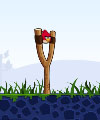
\includegraphics[height=3cm]{img/sling_detection_1}
	b) 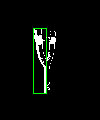
\includegraphics[height=3cm]{img/sling_detection_2}
	c) 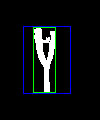
\includegraphics[height=3cm]{img/sling_detection_3}
	\end{center}
	
	\item[Edge cases] Before changing any parameters make sure to test it thoroughly with slingshots standing on various grounds (grass, wooden structure, hills, above air, below ground) and different birds in the sling (especially black and white birds). Another detection issue is high up in the clouds. One of the previous competition levels had the sling in the upper half of the screen.

\end{description}




\subsection{General Estimation Difficulties}

The open question is, can we calculate a perfect parabola prediction of the birds trajectory. Every scene is different, with a different scene scale and probably different flight characteristics per bird. How can we estimate the correct scale if the whole visual detection is prone to error? At least, we need a way to evaluate the trajectory after the first shot.


\subsubsection{Scene Scale and Magic Scaling Number}

Let's assume we already have a functioning trajectory estimation, but that estimation is limited to a fixed screen size. We need to transform the given calculations to a scene scale other then the optimized solution. We achieve that by computing a normalized scene. For this purpose we use the pixel scale of the already detected slingshot. In \class{database.Slingshot:getSceneScale()} the dimensions of the sling (width $+$ height) are combined into a single number. That number is what we simply refer to as \textbf{scene scale} (usually between \SIrange{55}{80}{px}).


Another scale, not to be confused with, is the \textbf{magic scaling number}. It can't be measured with the visual feature extraction. In fact the area defining the scene scale can be arbitrary. Looking at a level \texttt{.json} file we see two camera viewports `Slingshot' and `Castle'. By manipulating any or both viewports we identify that the scene scale is calculated somehow between these two. We don't know how the scale is calculated and more important even if we would, we couldn't access this information during runtime. This is where the \textit{magic scaling number} comes into play. Every time a shot is made, the predicted trajectory is compared against the actual flight parabola of the bird. Applying incremental updates to this magic number until eventually reaching the correct value. This number is usually somewhere between \numrange{0.95}{1.03}, stored in \class{meta.Level:scalingFactor} and reused upon revisiting the same level.


\subsubsection{Parabola Evaluation (after shot)}

As mentioned before we need to evaluate and compare the shot against our initial prediction. Luckily the game itself already draws the shot trajectory with small, white pixel clouds. Again, the original implementation in \class{ab.vision.VisionMBR:findTrajPoints()} uses quantized colors (\num{3} in this case) and Flood fill to extract the trajectory points (only taking pixel sets with max $5\times5$ px).

Our improved version \class{shot.VisionTraj} is not only extendable but also more accurate. Our version detects more clouds and at the same time includes less outliers. Furthermore the original version just took the center point of the pixel blobs bounding box. Our version computes the average point (or center of mass) under all contained points (the differences are noticeable). Finally, our method allows to split the trajectory point into a set before the tap and a set after the tap. Given that, we can utilize an autonomous shot evaluation for all bird types. Not only the default behavior but also their special capabilities and the resulting trajectory changes.

What's important to mention here is the process of filtering out outliers. First the point search is initialized at the trajectories pivot point (or at the tap point if searching for the special capability trajectory). Since we know the initial launch angle (or impact angle at tap time) we use this direction as starting direction. The next point on the trajectory (the next cloud) has to be within near distance. Also, the angle delta between the next and the previous point cannot change abruptly. From point to point the angle changes are subtle (\ang{+-23}).


\subsubsection{Launch Angle}\label{ch:shot:launchAngle}

An issue which took us quite some time to figure out, was the strange behavior of the original \class{ab.planner.TrajectoryPlanner}. Why is there even an attribute to adjust the launch angle by a small fraction (\numrange{0.025}{0.063}). Also why is this change not constant but depends on the launch angle itself. Our first guess was to rewrite the estimation completely and hope this adjustment will be gone for good. 
However, during testing even shooting with a fixed degree of \ang{45} will result in a shot that is not equivalent to the \ang{45}-shot. Even though the sent coordinates are $1000\times1000$ \si{px} away from the slingshot and the angle inaccuracy is neglectable. Turns out the game is doing some weird shit. As a consequence, we have to adjust each launch angle between shot estimation and shot execution. % lets see if this phrase will make it to the final document

The original implementation used this changeAngle multiple times throughout the estimation, whereas our version does one conversion at the end. As mentioned in the chapter introduction the original version relies on a \texttt{for} loop, whereas our version refines the angle with a recursive call. Most of the time the \num{2}. or \num{3}. iteration is already accurate up to \num{1e-5}.

But an other issue came up which is not present in the original implementation. Only because the original version has not the capability to do so. Our version has for each bird two equations. One for very-high-shots \ang{>75} and one equation for angles below \ang{75}. The very-high-shot equation is very steep so the recursive approach isn't suitable. We have to handle this case separately (see \class{shot.ShotHelper:estimateLaunchPoint()}). Furthermore, shots directly in the area where the two equations collide are probably estimated wrong (if starting with the wrong equation). Here, we have to find a better way to use both equations simultaneously.




\subsection{Class: ParabolaTester}\label{ch:shot:tester}

The \class{tester.ParabolaTester} class is the starting point for rapid prototyping and testing of new trajectory calculations. It provides a controlled environment with fixed, known slingshot dimensions and the corresponding pivot point. The mathematical equations are optimized for this specific scene scale. All needed resources are located in \source{/doc/parabolaEvaluation}.


\subsubsection{General procedure}

\begin{enumerate}
	\item To setup the environment load the \num{6} levels (\source{Level1-1.json}, etc.) into your game and change the boolean flag to \texttt{true} in \class{main.BamBird:main()}

	\item Run \class{ParabolaTester} and record raw data in \texttt{.csv} files in the root directory (all results are in the afore mentioned \source{/doc} directory).

	\item The raw file is then processed with the python script (\source{run.py}) into a readable format that is copy'n'paste accepted by Grapher (a macOS application).\\
	\textbf{Note:} If you want to omit this step, make sure you apply the same column calculations.

	\item In Grapher (or your application of choice) import the data and manually remove visible outliers (fig. \ref{img:shot:grapher}). Split the point set into separate groups with distinct features (e.g. everywhere where data points differ). Perform a curve fitting on all sets separately (Grapher: Select point set $\rightarrow$ Interpolation $\rightarrow$ Polynomial, Order 3).
	
	As seen in section \ref{ch:shot:launchAngle} we need an equation for the launch angle change and another equation for the velocity. Both equations take the launch angle (in radians) as input and output the corrected launch angle as well as the velocity needed to predict the parabola. Finally, we have to find the intersection point between the high shot and the low shot equation (Grapher: Select both equations $\rightarrow$ Menu Equation $\rightarrow$ Find Intersection).
	
	\item Save the results (Grapher \texttt{.gcx} file \& \source{fnGraphs.txt}) and export the data to Java.
\end{enumerate}


\begin{figure}
	\centering
	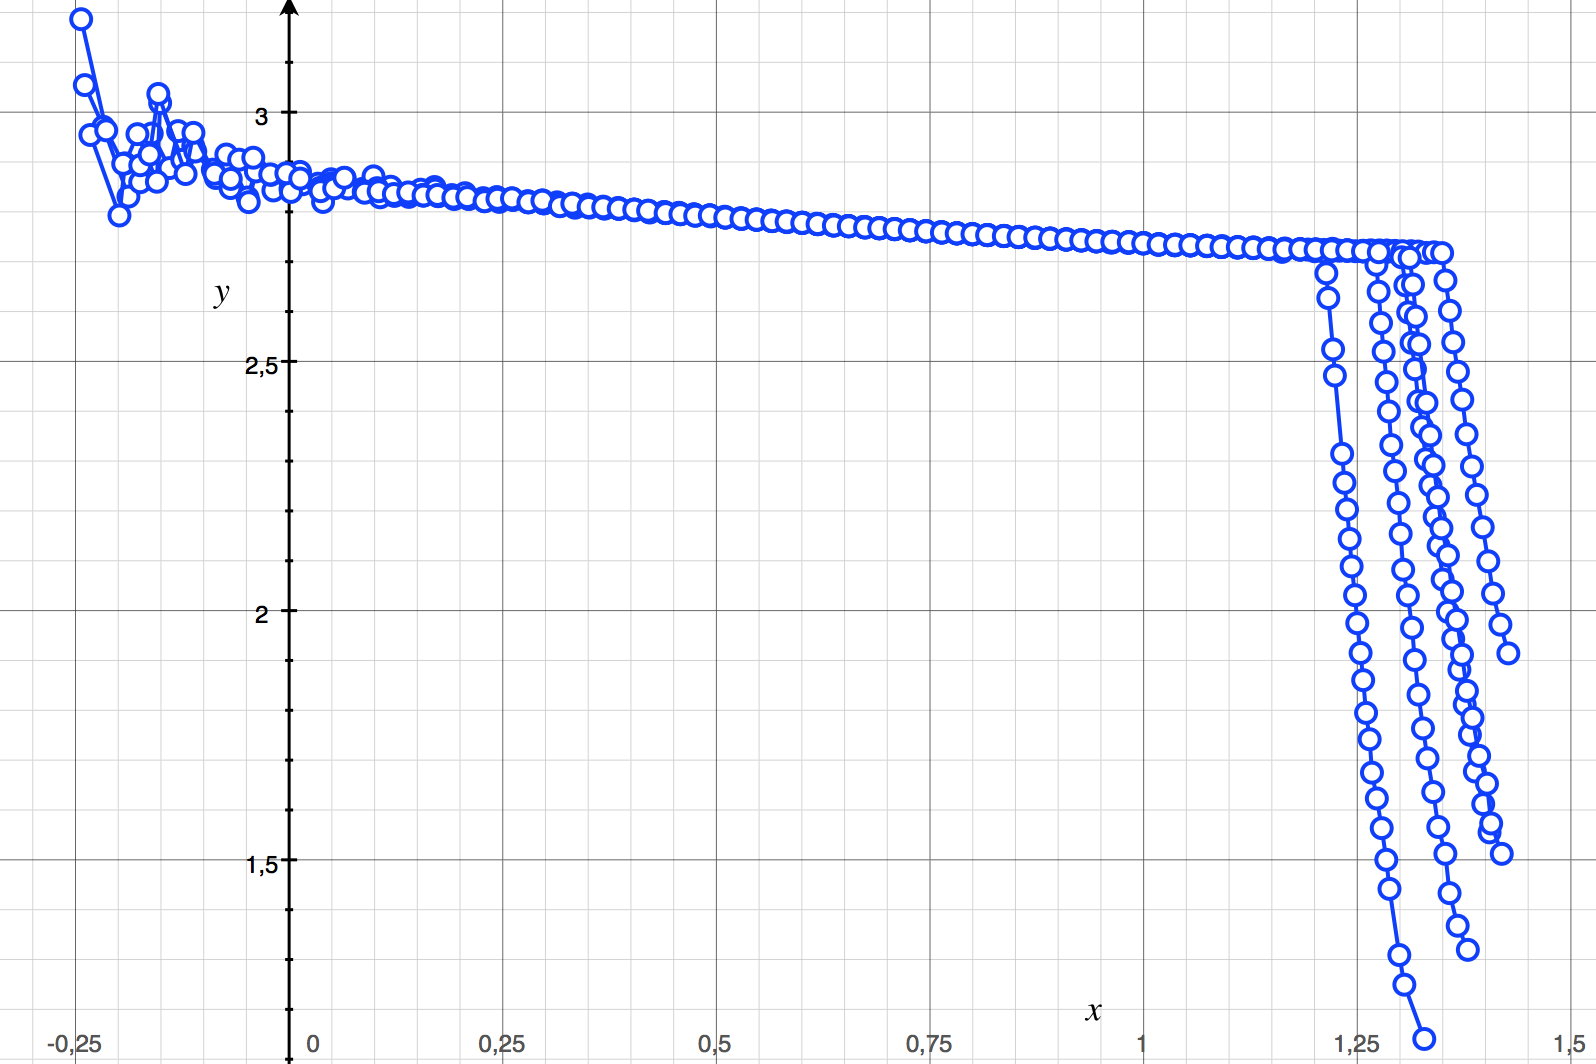
\includegraphics[width=12cm]{img/shotVelocity}\\
	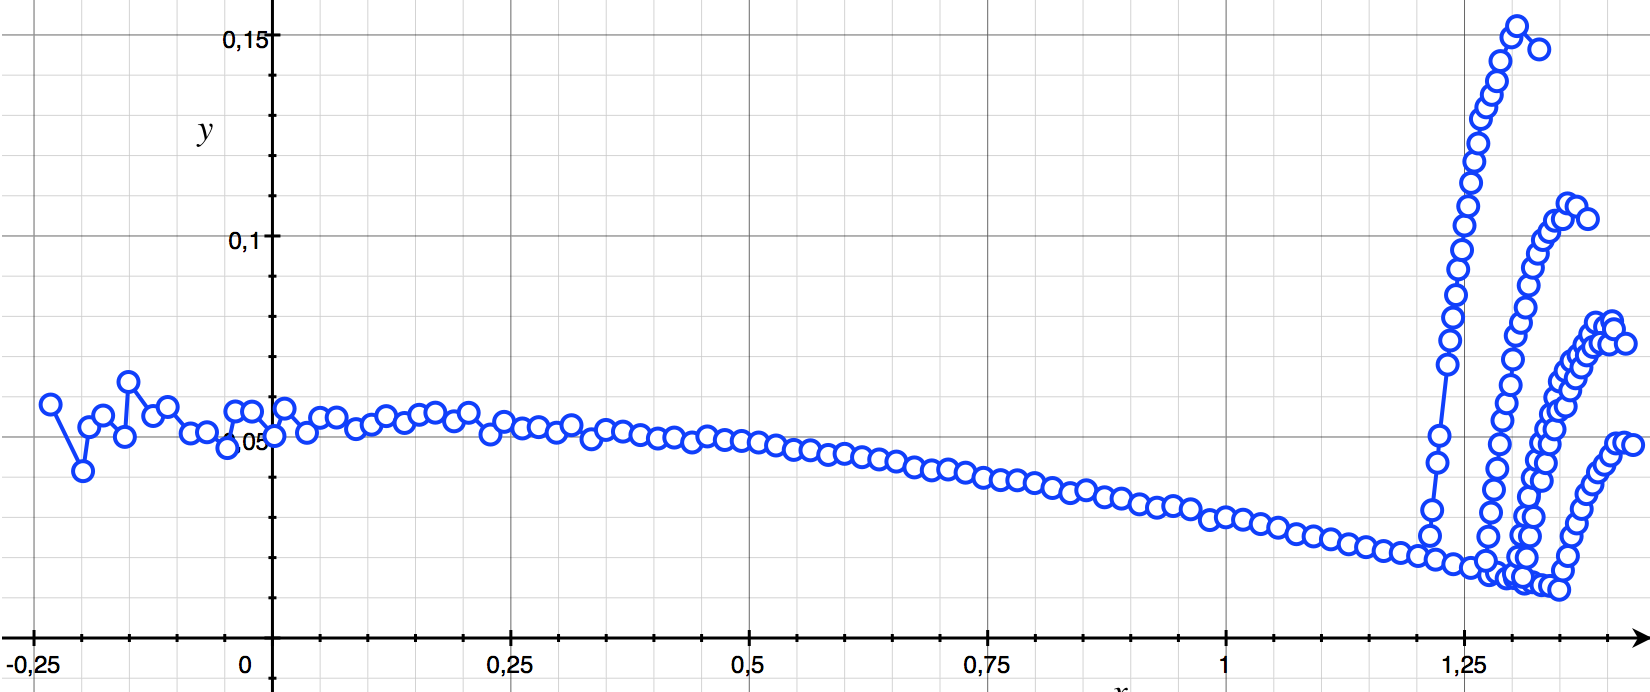
\includegraphics[width=12cm]{img/shotAngle}
	\caption{Raw data points for launch velocity (top) and adjusting angle (bottom) for all birds. X-axis: launch angle, Y-axis: velocity / change delta}
	\label{img:shot:grapher}
\end{figure}



\subsubsection{Different Testing Methods}

\begin{description}
	\item[\class{createShotEvaluationForAllBirds()}]$~$\\
	For all bird type try all shots between \SIrange{0}{86}{\degree}. Using \ang{1} steps until \ang{74} and \ang{0.5} beyond. Numerous tests have shown, that the low shots (red bird \ang{<74}, white bird \ang{<69}) are identical for all bird types. Therefore, this test will evaluate this range only once for the red bird. The very-high-shot ranges are evaluated for all birds nonetheless. The whole run takes roughly \SI{1}{\hour}.
	
	\item[\class{findAccuratePivotPoint(ABType)}]$~$\\
	Loads the level of the corresponding bird type and shoots at \num{4} different angles with \ang{10} spacing between. Each pair of two shots has an intersection somewhere in the slingshot area. This point is calculated and print to standard output (no file output!). Repeating this for all bird types will yield a (hopefully) accurate pivot point. All tests take \SI{5}{\minute}.
	
	\item[\class{findYellowBirdEstimation()}]$~$\\
	Similar to all birds evaluation the whole spectrum of the yellow bird special capability is covered. Testing impact angles (angle at tap point) from \ang{-65} to \ang{23}. Trying to shoot with different launch angles to add some variation. The result is somewhat unpredictable since it relies on a proper tap time estimation. However, the game server isn't very precise when it comes to tap time \dots This test alone takes \SI{38}{\minute}.
	
	\item[\class{shootRandomPoints()}]$~$\\
	Quick \num{9}-shot evaluation if the current equation parameter are accurate. Enable visual output (\class{DBG.enableDebug()}) to check if predicted parabola is identical to actual parabola.
	
	\item[\class{shootRandomPointsYellowTap()}]$~$\\
	Same as the test above but for yellow birds with automatic tap time estimation. \SI{1}{\minute}.
	
	\item[\class{shootYellowNear()}]$~$\\
	Does nothing yet. The idea was to predict a target point with normal trajectory estimation. Then adjust this given parabola slightly to the left to accurately hit the target even with yellow bird tap. With current implementation the yellow bird will always overshoot. 
	
	\textbf{Note:} This has to work independently of target position (even with impact angle \ang{>0})!
\end{description}




\subsection{Special Bird Estimation}

The parabola evaluation in section \ref{ch:shot:tester} has shed light onto boundaries of the original trajectory estimation. Because of the different bird sizes, very high angles will be cut at different angles for all birds (white: \ang{69} vs. blue: \ang{77}). Before version 2018 the special capabilities of different bird types were only considered rudimentary (blue: shoot ice, black: destroy as much as possible, yellow: go for wood). We are constantly moving closer to a full-featured tap-time prediction for all birds. Below is the current state of the software as well as some observations and suggestions on implementing the remaining estimations.


\subsubsection{Yellow Bird}\label{ch:shot:yellowbird}

We currently support only one type of yellow bird estimation. For a given target and a \textbf{fixed launch angle} we can estimate the tap point (\class{shot.ShotHelper:predictYellowBirdTapPoint()}). This approach will fail if the target can't be reached with the predefined launch angle. The tap-to-target trajectory is estimated as a straight line and refined successively (max \num{20} iterations) with the actual yellow bird equation.

Another type of yellow bird estimation (not implemented yet) is found by \textbf{refining the original parabola estimation}. The one calculated if no tap is happening (or `red bird estimation'). We already have a parabola estimation for the target without tap time. If the yellow bird is tapped (special capability activated) the bird will definitely overshoot and miss the target. On the other hand, we want to use the stronger shot gained from a tap. Therefore, we have to adjust the parabola to hit the target particularly with tap time. For near targets the launch angle needs to be adjusted more steep, whereas for far away targets the launch angle has to be lowered.

The third type for yellow bird estimation is \textbf{fixed impact angle} (not implemented yet). Sometimes we want to hit the target with a precise angle. For example, when an indestructable hill is blocking all other shot options (aka funnel). Although we don't see this type as very important, it could improve our performance in some rare cases tremendously.


\subsubsection{White Bird}

The estimation for white birds is rather simple. Start from the target you want to hit and go up in a straight line until you find a point that is hittable with normal estimation. This assures an egg-bomb will have a free fall to hit the target. Although currently implemented in Prolog, a Java implementation is missing. Depending on the future development, all estimations will be handled either in Prolog or Java.


\subsubsection{Black Bird}

The strategy for black birds is handled completely in Prolog. From the Java perspective we will always tap to make the bird explode. Prolog decides where the highest impact can be reached (and avoids black bird traps). We can still improve the prediction by allowing timed tapping. Sometimes its better to tap as early as possible, other times to wait until the bird explodes on its own. Pigs can be killed through hills if timed correctly.


\subsubsection{Blue Bird}

Although there is no blue bird estimation yet, a couple of observations: The middle path of the blue bird split will always stay unchanged. The other two paths split at the same angle in both directions. Also, since the middle path is unchanged, gives us a clue that the velocity doesn't change after the tap. Which in return means, that only the angle of the trajectory is changed in mid-air.

One option is to extend \class{tester.ParabolaTester} with an additional blue bird test. This includes clustering of the points after the tap into three groups (low, mid, high). The mid path can be found easily by extending the parabola before the tap. All other points lay either above or below this parabola. Points near the tap point and very high shots will distort the results (High shot: because the low split will project into the part before the tap and therein filtered out 'cause of abrupt angle change).

The second option is to manually try a few angles. Write a simple random blue bird tap shooter and experiment with fixed angles for both (high and low) splits. The velocity should be the same as the velocity at the tap point. Using the impact angle at tap point as base direction. Here again a piece of advice, the tap time isn't always accurate. A few bad runs don't necessarily mean the parameters are bad.




\subsection{Non-Working Alternatives}\label{ch:shot:fails}

This chapter summarizes all approaches we have tried but didn't led to success. Testing any further in that direction doesn't make sense, there are other areas to improvement.

We put a lot of effort into finding a solution that doesn't rely on adjusting the launch angle for each shot. One thing that doesn't affect the flight path is \textbf{gravity}. Changing the gravity for different birds is the same as having a unique equation per bird. Nonetheless all calculations in \class{helper.ParabolaMath} respect the gravity constant. Though the static variable \texttt{\_g} is fixed to \num{1.0} (compiler optimization will ignore the unnecessary calculation anyway).

Also searching for a solution that better reflects the slingshots \textbf{pivot point} is wasted time. The current solution is accurate up to \num{4.5e-3} on relative values (\numrange{0.0}{1.0}, value $\times$ sling width). Instead of tweaking the parameters in \class{database.Slingshot:calculatePivot()} (generated by \class{tester.ParabolaTester:findAccuratePivotPoint()}), we need to optimize the detection of the slingshot. If the detected rectangle is faulty, the resulting pivot point will vary heavily. We can't be sure that neither the slings height, nor the slings width will be detected correctly. Currently, the height is ignored because in many test levels the sling was lowered too deep into the ground. A size independent slingshot detection isn't feasible yet, since the scene scale relies on that measure too.


\textbf{One calculation for all bird types} would be the preferable solution, especially for high shots. But experimenting with various settings, there is no rule between the birds size and the very-high-shot change angle. Of course there is, but non that is eminent and can be used with the available information. Theoretically the bird size should influence the high angle cutoff exclusively. However, the real bird sizes (\class{database.ScreenScale}) dont't even have the same ratio as the in-game bird sizes. In theory, the high angle cutoff should be a straight line, instead the line is slightly bend (compare fig. \ref{img:shot:grapher} top).


\section{Strategy Improvements}\label{ch:strategy}

\subsection{Decision Tree}\label{subsec:decisionTree}
If the agent loses a level and re-enters it again at a later point of the competition, it should not try the same consecutive shots, that lead to failure in the first try, again. In order for the agent to gain knowledge about wether a shot led to failure or pass of a level, a decision tree was implemented (see \texttt{DecisionTree.class}). This way, the second, third or nth time the agent retries a level, it should not do the same bad shots over and over again. The decision tree is only of use in lost levels. It has no effect on levels that have already been won. It could, however, in future work be implemented so that if an already won level is retried, the agent will not do the exact same shots again, but try something new and see if it gets more points.

\subsubsection{Functionality of the decision tree}
Every time the agent enters a level for the very first time, a single instance of a tree is saved within the level representation of that level. Every time the agent re-enters a level, its already existent tree instance reloaded. Every time the level is being played, the same tree instance gets modified.

The root node of the tree is the situation the agent is in when it enters a level. Soon enough, Prolog calculates the options for the next shot and returns them to the agent. Each of those options represents a new node in the tree structure. The agent picks one of the options, shoots, and the respective node for that shot becomes the representation of the current situation and the node gets marked as \textit{visited}. Now, another set of possible next shots is calculated, new nodes are added and so on. In fig \ref{fig:take1}, the nodes on each level of the tree represent all options after one shot. The blue nodes represent shots that the agent decided to take, one after the other.

In the assumption that the last shot that is being conducted leads to losing the level, this node gets marked as \textit{lost} (see fig. \ref{fig:take1}). The tree is designed so that it never takes a shot that would lead to being in a situation that is marked as \textit{lost}. This means, that if one parent node has e.g. two childnodes, and, in a second attempt to win the level, both of them are lost, the parent node will also be marked as lost, as there is no way of winning the game if this node's shot is taken (see fig. \ref{fig:take2}).

\begin{figure}
	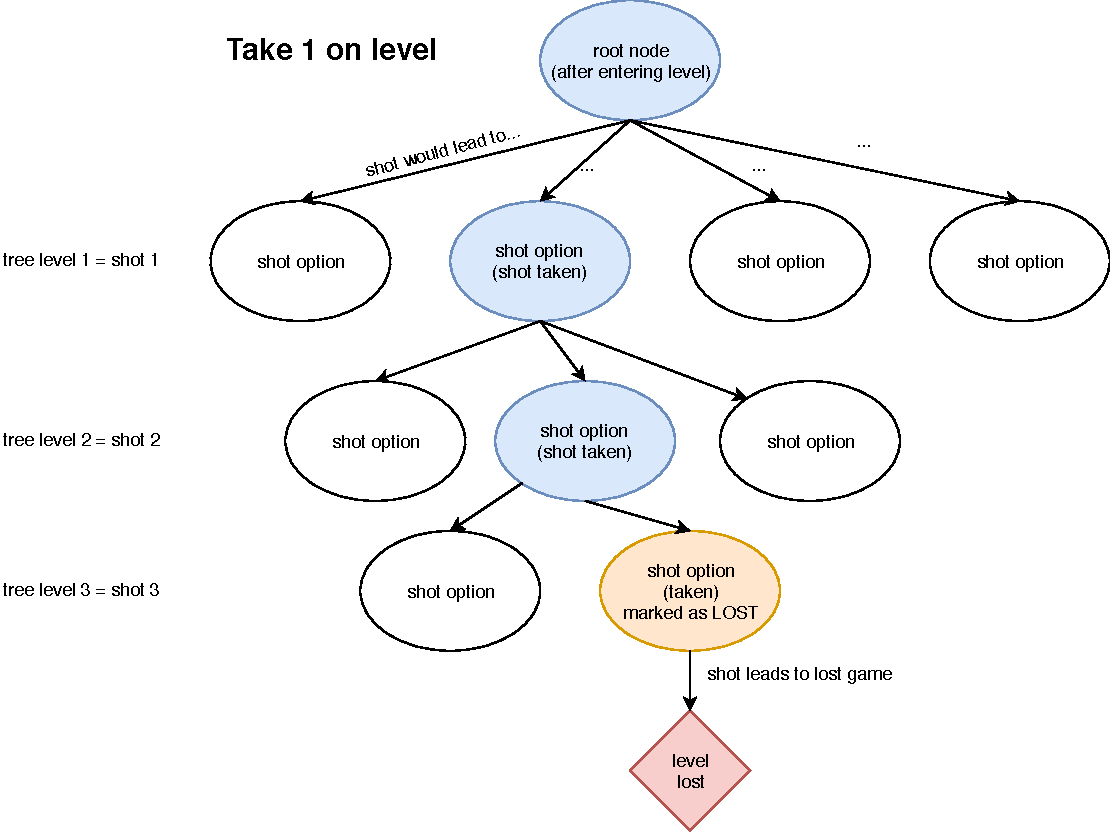
\includegraphics[width=\textwidth]{img/take1onlevel.pdf}
	\caption{First attempt to win the level ends with a lost game. The last node (which represents the shot that used the last bird) is marked as \textit{lost} and will never be taken again.}\label{fig:take1}
\end{figure}
\begin{figure}
	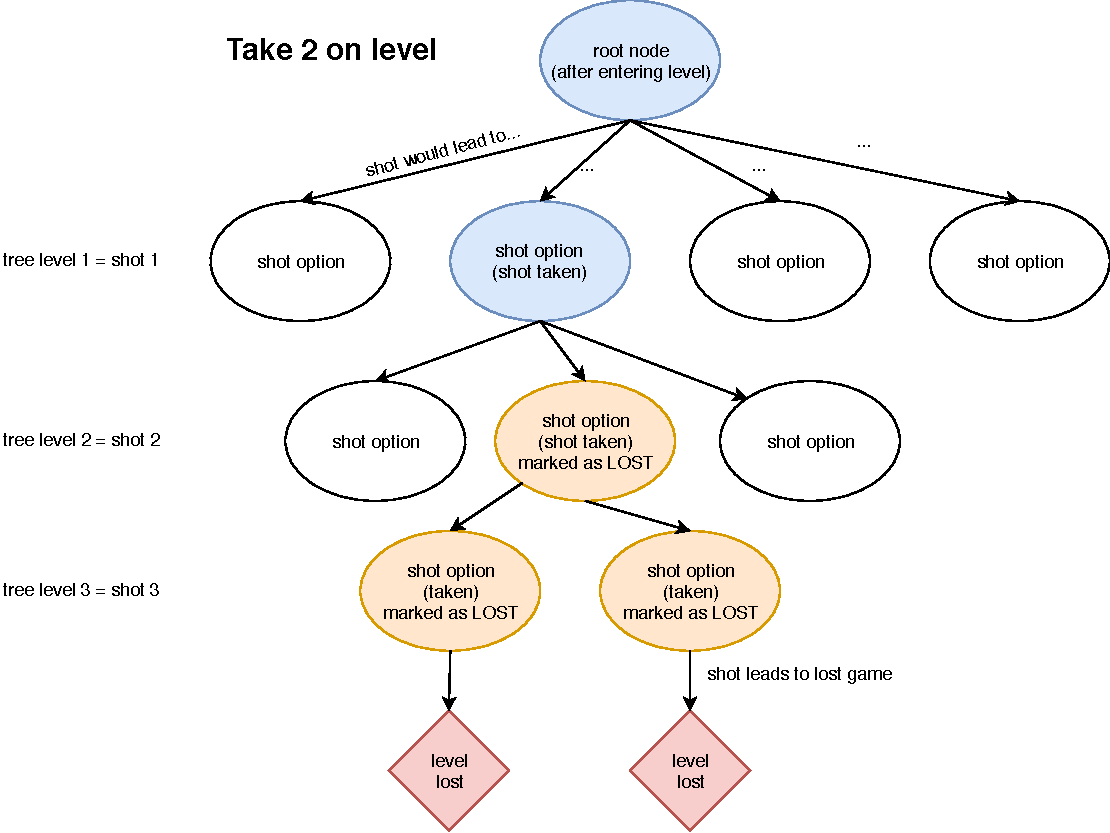
\includegraphics[width=\textwidth]{img/take2onlevel.pdf}
	\caption{In this example, the shot path in the second attempt stays largely the same. Since all two child nodes of the taken shot on level 2 led to lost games, the node on level 2 is also marked as lost.}\label{fig:take2}
\end{figure}

\subsubsection{Backpropagating negative impact for the confidence of a shot}\label{subsec:backpropagationConfidence}
Whenever Prolog calculates the options for the next shot, it provides the agent with a list with all possibly successful shots. Those possible shots all have a confidence rating, which expresses how successful Prolog predicts the shot would be. The agent currently picks its next shot according to the shot with the highest confidence rating. If a shot leads to a loss, we backpropagate a negative impact on this confidence all the way back to the root node for every shot that had been taken on the way to losing the game. This impact starts with \(-0.5\) for the parent of the lost node (see fig. \ref{fig:negativeImpact}. The impact is being divided by two for every node on the way back to the root node. This way, the agent will be encouraged to decide for a different chain of shots before it is in a situation that will likely lead to a loss again.

\begin{figure}
	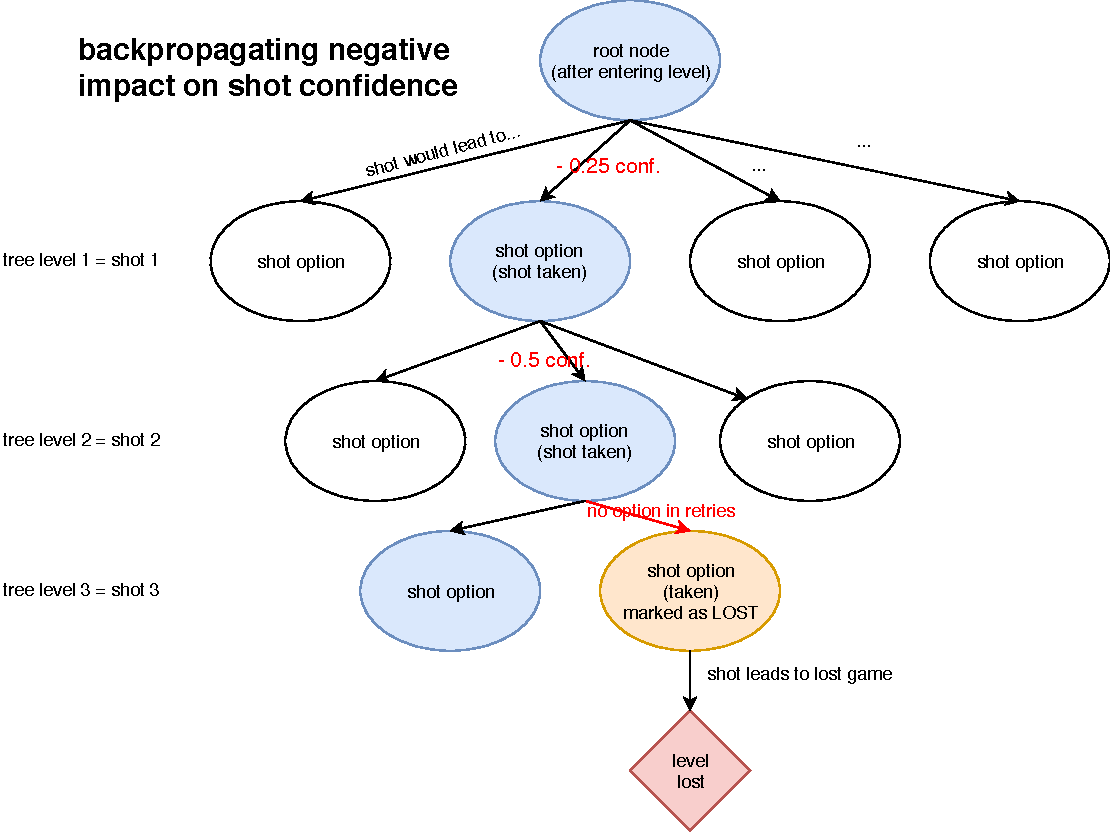
\includegraphics[width=\textwidth]{img/negImpact.pdf}
	\caption{Backpropagation of negative impact of a loss. The impact starts at the parent of the lost node, since the lost node itself will never be re-entered again anyway.}\label{fig:negativeImpact}
\end{figure}

\subsubsection{The problem of randomness in the physics of the game}\label{subsec:randomnessInPhysics}
If the agent enters a level twice, the same best shot is calculated twice and the same shot is taken twice, one would assume the level on the first attempt looks exactly the same as on the second attempt. However, there is a small randomness in Angry Birds' physics. This means that sometimes, when a level is entered for the second time, one can not be sure that if the same shot is taken, the tree would look the same as the first time. In order to prevent the tree representation of the game situation looking different than the actual game situation, after each taken shot, the current situation's screenshot is being compared to the screenshot of the previous attempt. If the level looks different despite having taken the same shot, the current situation will be saved in the tree inside a newly created node.

\subsubsection{Shots that have no effect}\label{subsec:shotsThatHaveNoEffect}
If the agent shoots e.g. onto a concrete terrain block, no damage is done by that shot. This means that the level will also still look the same. That shot then was completely wasted. In order to prevent the agent from taking repeatedly shots that do not change the situation, each time a shot is conducted, the situation after that shot will be compared (by comparing the blocks' positions) to the situation before the shot. If the level still looks the same, a new node will be appended to the current node that is marked as \textit{lost}. For every shot the agent takes, it checks beforehand if the current node has a child node containing the exact same shot. In this case, this would be true, and that node would also be marked as lost. This shot would then not be taken.

%The slope detection is on it's onw branch, and has not been merged with the master branch. 
%This is mostly due to a lack of testing.
\subsection{Slope Strategy}\label{subsec:slopeStrategy}
So far, the Agent has ignored "Heavy Objects", like large stone boulders, completely, excluding cases where they were directly above a 'priority target', aka a pig or TNT. Several Angry Birds levels contain such Boulders on the top of hills, or on a slope, blocked by a destructible object. The new slope detection checks several positions around boulders for contact with the ground, or a hill, and determines if the boulder in question could be made to roll down a hill. If so, the agent will treat it similarly to heavy objects above pigs or TNT. \linebreak
As there is no support for complex interactions, it will not check for priority targets to the left of heavy objects of hilltops, as the agent has no means to nudge a boulder to the left while shooting from the left, and pigs on the left of a hill can usually be hit directly.
\ref{fig:Dec_Tree}
The agent checks the position of heavy objects if the vision module reports that they are resting on a hill. It does so by checking for collision of the bottom left and bottom right of the boulder's bounding box, which the vision module provided, to check for uneven ground, then checks for ground contact to the left and right of the object to detect a hilltop position. 
\ref{fig:slopeEx}
Currently, the slope detection does not check for multiple objects between the Heavy Object and Priority Targets.
\begin{figure}
	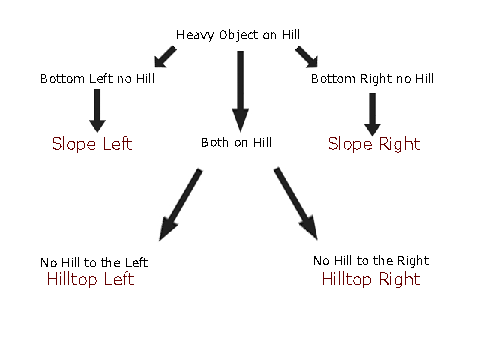
\includegraphics[width=\textwidth]{img/Dec_Tree.pdf}
	\caption{Decision tree to check for slopes. Heavy Objects on actual slopes do not need to check for hilltops in the same direction.}\label{fig:slopeEx}
\end{figure}

\begin{figure}
	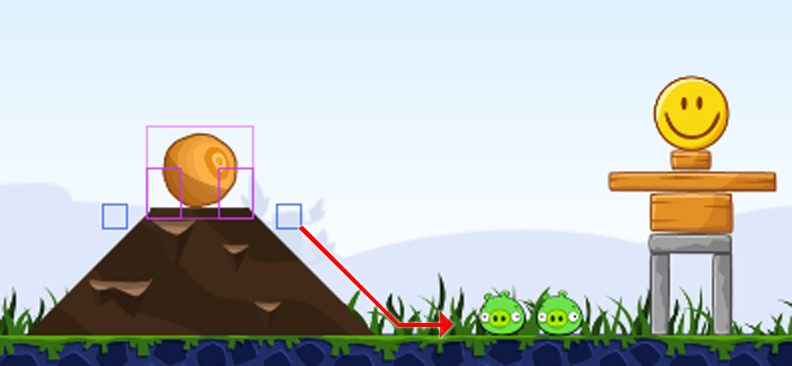
\includegraphics[width=\textwidth]{img/shot1hr}
	\caption{Slopecheck: The Heavy Object is sitting on a hilltop.  In this example, there is a priority target to the bottom right of the boulder, indicating the boulder as a potential target for a direct shot.}\label{fig:slopeEx}
\end{figure}

% this has not been implemented. It might be in the future though, after further evaluation.
\subsection{Weka Machine Learning \textit{not implemented yet}}
Disclaimer: this option of further improvement of the agent has not been implemented yet. It might be helpful in the future, though. Further investigation and evaluation is required. This chapter is just a description of current findings.

\subsubsection{Introduction}
Weka is a collection of machine learning algorithms for data mining tasks. It includes methods for data mining problems such as regression, classification, clustering, association rule mining, and attribute selection \footnote{Eibe Frank, Mark A. Hall, and Ian H. Witten (2016). The WEKA Workbench. Online Appendix for "Data Mining: Practical Machine Learning Tools and Techniques", Morgan Kaufmann, Fourth Edition, 2016.}. Weka is used by applying a learning algorithm to a given dataset and analyzing its output. Another way of using Weka, which is relevant for our use in BamBird agent, is to generate predictions on new instances, and a third way is to apply different learning algorithms and compare their outputs and performances.

\subsubsection{Implementation}
For the use in BamBird, Weka is used to classify a new instance. The class to be learned is whether a shot is good or bad, this is called a relation in Weka. This relation is dependent on attributes, and the attributes for the BamBird agent are, strategy name, confidence class, damage points and pigs killed. Weka uses an ARFF \footnote{https://www.cs.waikato.ac.nz/ml/weka/arff.html}. file. The ARFF file contains two sections, the header section and the data section. We give a brief description. Below we show the header of the ARFF file. The header contains the relation, a list of attributes and their data types.

The header section of the ARFF file looks like this:
\begin{lstlisting}
@relation good-shot
@attribute strategy-name 	{targetPig ,domino, blackBird,
collapseStructure, tnt, heavyObject, whiteBird}
@attribute confidence-class	{A, B, C}
@attribute damage-points	REAL
@attribute pigs-killed		REAL
@attribute class		{good, bad}
\end{lstlisting}
\ \\
The header section of the ARFF file is followed by the ARFF Data Section. It contains the data declaration line and the dataset. Below we show a snapshot of our training dataset. Default values from section 4.1 are used to mark a shot as good or bad. Confidence class is identified as follows: class A from 0.5 to 0.6, class B from 0.6 to 0.9 and class C from 0.9 to 1.0. The Data Section looks like this:

\begin{lstlisting}
@data

domino,C,0,0,bad
domino,C,0,0,bad
targetPig,C,8760,2,good
domino,C,16100,3,good
targetPig,C,5320,2,good
targetPig,C,12530,3,good
targetPig,A,1160,0,bad
targetPig,A,6440,2,good
heavyObject,C,32580,6,good
\end{lstlisting}
\ \\
In order to classify a new instance, a new ARFF file is created at runtime, called \texttt{unknown.arff}. The header of \texttt{unknown.arff} is the same as the header described above, but the data section is different. Instead of having an entire dataset, only one data is provided, described below.
\ \\
\ \\
\texttt{targetPig, A, ?, ?, ?}
\ \\
\ \\
The \texttt{?} is the dataset signifies unknown data. To classify this instance, we know that the strategy is \texttt{targetPig} and we know that the \texttt{confidence-class} is \texttt{A}, but \texttt{damage-points}, \texttt{pigs-killed} and shot \texttt{class} are unknown. We use the NaiveBayes algorithm as implemented by Weka to classify this new instance.
\ \\
\ \\
Following we present the updated \texttt{Meta} algorithm for Weka and the \texttt{ClassifyShot} algorithm.

\begin{algorithm}[H]
	\SetAlgoLined
	load the ShotLearner database\;
	\While{true}{
		\If{GameState != Playing}{
			choose new Level using the new equation\;
		}
		take a screenshot from the scene and analyse\;
		generate plans\;
		select the first Target from the plans and send it to WekaTester\;
		WekaTester classifyShot marks the Target good or bad\;
		\uIf{goodTarget}{
			execute the seleted shot\;
		} \uElse{
			remove the target from plan\;
			go to 8.\;
		}
		add shot to the shot-list of the current level\;
		\If{GameState == WON or GameState == LOST}{
			add level to database\;	
		}
		add the shot to ShotLearnerDatabase\;
		create a ShotResult object with the results of the shot\;
		save the ShotResult to a log file\;
	}
	\caption{Meta-Updated} \label{algorithm:metaUpdated}
\end{algorithm}
\ \\
Line 7 – 14 mark the difference in the updated \texttt{Meta} algorithm. A \texttt{Target} is selected from the generated list of plans and is sent to \texttt{WekaTester}, where this target is transformed into an instance and written to \texttt{unknown.arff} file.
\ \\
\ \\
\begin{algorithm}[H]
	\SetAlgoLined
	create unknown.arff file\;
	write the header\;
	transform target into ARFF data instance\;
	invoke NaiveBayes classifyInstance and save into prediction string\;
	return prediction string\;
	
	\caption{Weka: ClassifyShot}\label{algorithm:classifyShot}
\end{algorithm}
\ \\

There are two points of interest in Algorithm \ref{algorithm:classifyShot}. The first is the transformation of \texttt{Target} object into ARFF data instance. This is trivial and is achieved by string manipulation and string writing onto the \texttt{unknown.arff} file. The second interest point is the invoking of \texttt{classifyInstance} of \texttt{NaivesBayes} algorithm. This is also trivial because the logic is abstracted behind a simple method call, shown below.
\ \\
\ \\
\texttt{double predNB = nb.classifyInstance(newInst);} \footnote{http://weka.sourceforge.net/doc.stable/}
\ \\
\ \\
where \texttt{predNB } is the predicted class, \texttt{nb} is the instance of \texttt{NaiveBayes} class algorithm and newInst
is the new data instance that we wish to classify and predict the class of.
\ \\
\ \\
Implementing learning algorithms from Weka promise to be of use for the BamBird agent, but have not been implemented yet.

\section{Miscellaneous}\label{ch:misc}

\subsection{Including a logger for debugging}\label{subsec:logger}
The agent gives multiple lines of output during its gameplay. Some of it is only necessary during development, but not during the competition. Text outputs also require (a quite small amount of) cpu time. In order to save this time and declutter the agent's output during the competition, we implemented a \texttt{CustomLogger.class} that instanciates a \texttt{java.util.logging.Logger} and a custom message formatter. It listens to the constant \texttt{DEBUG\_ENABLED} inside the \texttt{Constants.class}. If this value is set to true, every message of the agent will be printed. If it is set to false, only messages that are marked as \textit{warning} or \textit{severe} will be output.

In order to keep this ability, no more \texttt{System.out.println()} calls should be used. Instead, one should use \texttt{CustomLogger.[info/warning/severe]([message string])} in order to output messages. One can also, at any time, call \texttt{CustomLogger.setLevel(["info"/"warning"/"severe"])} in order to change the log level. Since the logger is implemented as a singleton, every class that instantiates a \texttt{CustomLogger} object will work on the same instance.\\
On starting the agent, in \texttt{BamBird.class} the function \texttt{CustomLogger.saveLogsToFile()} is called. This effects that every message will be output, but also saved in \texttt{logfile.log}. 

A typical output of the logger would be

\ \\
\begin{centering}
\texttt{[2018-08-10 15:12:30] [INFO] meta.Meta | Choosing new level ... } \\
\end{centering}
\ \\
It shows a date- and timestamp, \texttt{[INFO]} marks the log level, \texttt{meta} is the package and \texttt{Meta} the class from which the logger is called, followed by the actual message "\texttt{Choosing new level}".

\subsection{Documentation tool}\label{subsec:code documentation}
For a clear dokumentation there is the posibility to use the documentation generator 'Doxygen'. Hence it is necessary to install Doxygen and GraphViz. To build the documentation you have to open your terminal/bash in the documentation directory and run 'doxygen configfile'.
The configfile is a default by our project group but you can also tweak the settings by yourself. Therefore you have to use 'Doxywizard'(Open the terminal/bash and run 'doxywizard'). The graphical user interface is easy to handle and settings can be changed\footnote{https://www2.informatik.hu-berlin.de/swt/projekt98/werkzeuge/doxygen/Doxygen.html}.
The documentation in the programming code has to keep some rules: \\

Writing '/**' and enter creates automatically the main functions like: \\
@brief - short brief of the code \\
@param - description of the parameter \\
@return - description of the return value \\
@class - description of the class \\

Further information on how to use doxygen can be found in the following document\footnote{http://www.vislab.de/cgbuch/intros/doxygen.pdf}.
\section{Open Tasks for 2019}\label{ch:todo}

% Whatever we coudn't finish and hope the next team will tackle.
% Be as specific as possible, this makes it easier for the next team to start ;)

This chapter summarizes our key findings and things that are left undone. Below just a listing of possible tasks for the next project group:

\begin{description}
	\item[Fix `no retry after 3 failed attempts']
	During the finals in the last competition our agent couldn't complete \num{5} out of \num{8} levels. Current level selection strategy (\class{meta.LevelSelection}) will try every level three times. If we couldn't complete the level by then, it will load an already played level and try to improve the score. However, this makes absolutely no sense in the competition environment. Moreover the complete level selection strategy should be revised as the current selection is rather linear.
	
	\item[Better handle crowded scenes]
	Another very critical task is the performance in crowded scenes. Our agent performed worst in situations where the scene contained a lot of objects. Other (simulation) agents achieved high scores in those levels whereas our agent couldn't even complete with a low score. Currently the target point reachability calculation (\class{features.Scene:setReachabilityForAllBlocks()}) will create up to \num{5} targets per object. Besides a potential performance loss, this behavior may influence Prolog's decision making; too many targets distraction. Future versions should stick to just a single target per object (if there are many objects in the scene). Furthermore, the Prolog strategy needs some major adjustments to identify targets with similar behavior. Or even better, let Prolog do the reachability calculation only for those targets that are important.
	
	\item[Prolog parabola estimation]
	As mentioned before the reachability calculation can be moved to Prolog entirely (partially already done). Whats left undone is to restructure the communication flow Java $\leftrightarrows$ Prolog. Currently, Java runs some image processing, calculates reachability for all objects, creates a \source{situation.pl} file describing the scene, and starts Prolog to evaluate the options. There are two options to improve the message flow. Either find a way to communicate both ways directly (instead of an indirect Prolog call); Or start the communication from the Prolog part. Java will only run the image processing and write a scene description. Prolog then calculates the reachability for important targets only and sends the target list to java to perform the shot.
	
	\item[Scene scale by considering all objects]
	Current scene scale estimation relies on a robust detection of the slingshot (width and height). The idea was to use all scene objects' dimensions instead. More objects means also more errors during detection. Since we know how big the objects should be a clustering algorithm can group similar sizes together. The overall uncertainty should decrease with more measures (at least thats what we hope for).
	
	\item[Parabola equation overlap]
	An issue described in section \ref{ch:shot:launchAngle} may produce wrong parabola estimations. Since all birds have two equations (one for low and one for very-high shots) the launch angle area between those two equations may be incorrect. We didn't have the time to look deeper into this. Currently, the launch angle refinement is done in either one of these equations. But after selecting one we will not check if the best solution is in fact in the other one.
	
	\item[Yellow Bird target correction]
	As described in section \ref{ch:shot:yellowbird} the yellow bird estimation needs to be adapted to allow parabola correction. Also, finding a use for the implemented, but not used, fixed-angle-estimation.
	
	\item[ClientActionRobotJava]
	We use \class{meta.ActionRobot} to handle the Client-Server communication. Our robot is a subclass of \class{ab.demo.other.ClientActionRobotJava} and doesn't support going from the main menu to the level selection (all other agents from the competition do). However \class{ab.demo.other.ActionRobot} has this functionality built-in. Adopting the changes from the latter one to our solution; Or rewriting our robot to be a subclass of the latter one is an open task.
	
	\item[Random Levelgenerator]
	In section \ref{Random LevelGenerator} we described the random levelgenerator with its different types of levels.
	Currently the different structures cannot be combined in one level this is a goal that should be achieved in the future. The birds the client can shoot with are four red birds but need to be adapted to the structure, the type of pigs and the material in the generated level. Additionally, it should be possible to position the random blocks around the different structures without destroying them. For this we wanted to use an array that contains the used x-values so the random blocks, pigs and terrains are not colliding with the structure. If the structure is off the ground it would be helpful to track their height aswell. This allows to put random things on the ground if the structure is above it and if multiple structures are put together in one level later on it can be seen if they collide (in the air and on the ground).
\end{description}


\end{document}
